\section{Chapter Overview}
This chapter explains the core implementation of the research prototype together with the technologies, languages \& supporting tools used for development of the prototype, with reasoning to the choice of each selection.

\section{Technology Selection}

\subsection{Technology Stack}
The technologies that were used to implement the prototype at each layer are shown below.
% Technologies used in various tiers or layers using a diagram.

% canva design: https://www.canva.com/design/DAEr30kH33k/mLBvcR5DptGOwK55cJddvA/edit

\begin{figure}[h!]
\centering
\frame{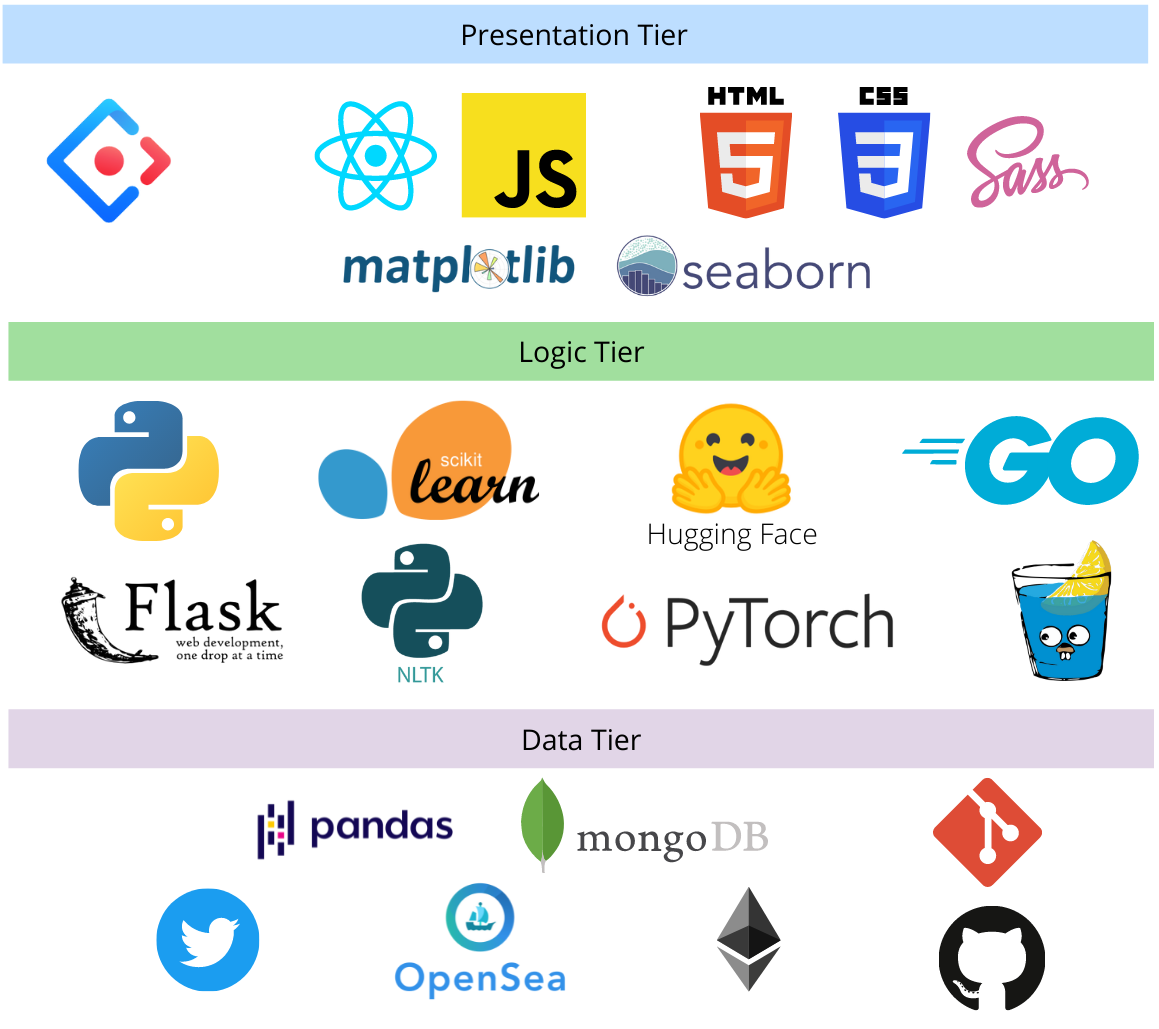
\includegraphics[width=0.8\textwidth]{images/Implementation/tech-stack.png}}
\caption{Technology Stack \textit{(self-composed)}}
\label{fig:teck-stack}
\end{figure}

% TODO: add a description (if not described later)
% \blindtext

\textbf{Linux} will be the default choice for development since of the ease of support for multiple development tools and performance benefits. MacOS/ Windows will be used for research documentation \& study purposes.

\noindent The rest of the choices in the above tech-stack have been explained in the following sections.

\subsection{Data Selection}
% Data Selection (if data science project)
Being a data science project at the core, it was important to choose the best possible sources of data to gather sufficient data for analysis \& produce the best possible recommendations.

The data requirements identified were,
\begin{enumerate}
\item \gls{nft} asset data
\item Global trends data
\item \gls{nft} Smart Contract data
\item \gls{nft} events (sales) data
\item \gls{nft} bids data
\end{enumerate}

Since the main technological research gap to be addressed was with the integration of global trends into content based recommendations, this was given a higher priority at first.
These data requirements were sourced from the following sources and heavily pre-processed there after to create a usable dataset for data analysis. 

\begin{itemize}
\item \gls{nft} asset, events, bids data - From the \textbf{OpenSea API}.
\item Global trends data
\begin{itemize}
    \item Twitter data - From \textbf{Twitter developer API}.
    \item Google Trends data - From Google Dataset Search \& unofficial \textbf{Google Trends Python API (Pytrends)}.
%     \item Reddit data - From the Reddit API.
\end{itemize}
\item Ethereum Smart Contract data - From Etherscan \& OpenSea
% \item \textbf{User Preference Profiles data} - From Amazon, Yelp, Kaggle open datasets. May be needed for testing purposes.
\end{itemize}


All the data-points that could be used for recommendations and explored with iterative development, as a research. This iterative process took a long time since the \gls{api}s were rate limited. The gathered pre-processed datasets will be made available for public use for future researches.

\subsection{Selection of development framework}
% Use a table to justify your selection for each of them.
\vspace{-4mm}
\begin{longtable}{|p{0.16\linewidth}|p{0.8\linewidth}|}
\caption{Selection of development framework}\\ 
\hline
\textbf{Framework} & \textbf{Justification for selection}\endfirsthead 
\hline
Gin Gonic & It's extremely convenient to build \gls{api}s using Gin with Golang. It also has an easily debuggable log output \& claims smashing performance (up to 40 times faster!)\\
\hline
Ant Design & The world's second most popular React UI framework. Used in many industrial applications and has a wide range of components to match most UI requirements. Since it's tree-shaking compatible, it will build only the components that are used. This reduces build time of the frontend. The CSS is easily customizable as well. \\ 
\hline
\end{longtable}

Although this is a data science project, all data science models utilized were built from scratch without the use of libraries, since doing so allowed the author to tweak the models at will.

% -----

\subsection{Programming language}
% Justify what you’re using, why you’re using it.
\textbf{Python} is the language that will be used to create the \gls{ml} models.  Python is an all-purpose language that has been used in many projects involving data science. It has a vast collection of supporting libraries that eases many data science related tasks.

For the \gls{api} proxy it was decided to use \textbf{Golang}, which is statically typed language that attempts to resemble the performance of C. Golang will allow the application to support concurrency and multi-threaded communications while being extremely lightweight and fast. This will be used to avoid any bottlenecks that could occur at this point in the system, while potentially bolstering performance.

For the frontend, \textbf{JavaScript} was decided to be used to show dynamic content and allow a highly interactible \& inviting user experience.

\subsection{Libraries Utilized}
% Tabular form and justify.
\vspace{-4mm}
\begin{longtable}{|p{0.16\linewidth}|p{0.8\linewidth}|}
\caption{Libraries Utilized with justification for choices}\\ 
\hline
\textbf{Library} & \textbf{Justification for selection}\endfirsthead 
\hline
% data science python libraries used
Pandas & Pandas dataframes allow a vast range of functionalities required for data analysis such as cleaning, transforming, filtering, sorting \& manipulating of data \\
\hline
Scikit-learn & Used for vectorizing text and generate similarity matrices between items, for recommendations. \\
\hline
NLTK & Convenient to use for \gls{nlp} data parsing, using the RAKE vectorizer. \\
\hline
SpaCy & Allows production-ready advanced \gls{nlp}. \\
\hline
Beautiful Soup & Convenient to scrape data from the internet. \\
\hline
Matplotlib & Has almost any type of visualization method for data analysis. \\
\hline
React & A UI library that makes it easy to build interactive websites. Used as an alternative to using a framework since the vast array of capabilities and other integratable frameworks and libraries. It was important to develop an easily interactible frontend, since it will be the users’ point of interaction with the system. \\
\hline
\end{longtable}

% \pagebreak
\subsection{IDE’s Utilized}
% Tabular form and justify.
\vspace{-4mm}
\begin{longtable}{|p{0.16\linewidth}|p{0.8\linewidth}|}
\caption{IDEs Utilized with justification for choices}\\ 
\hline
\textbf{IDE} & \textbf{Justification for selection}\endfirsthead 
\hline
Google Colab & Convenience of trial \& error of fetching data, building, testing \gls{ml} models and ability to work across multiple devices with the cloud development environment. \\
\hline
VSCode & Extremely dynamic while being simple to use, yet powerful for front-end development with it's extensions \& code snippets. \\
\hline
Golang & Convenient syntax highlighting \& auto-completion for Golang development. \\
\hline
PyCharm & Well-equipped Python \gls{ide} with a lot of capabilities.\\
\hline
\end{longtable}


\subsection{Summary of Technology selection}
% tabular form
\vspace{-4mm}
\begin{longtable}{|p{0.3\linewidth}|p{0.65\linewidth}|}
\caption{Summary of Technology selection}\\ 
\hline
\textbf{Component} & \textbf{Tools}\endfirsthead 
\hline
Programming Languages & Python, Golang, JavaScript \\
\hline
Development Framework & Gin Gonic \\
\hline
UI Framework & Ant Design of React \\
\hline
Libraries & Pandas, Scikit-learn, NLTK, SpaCy, Beautiful Soup, Matplotlib, React \\
\hline
IDE – Research & Google Colab \\
\hline
IDE – Product & VSCode, Golang, Pycharm \\
\hline
Version Control & Git, GitHub \\
\hline
Application hosting & Netlify, AWS
% Google Cloud App Engine?
\\
\hline
\end{longtable}


\section{Implementation of Core Functionalities}
% Discuss core functionalities with support of code segments.

Since a Recommendations System's ultimate goal is to reduce the amount of information overload and provide the user with the best possible options, it was essential to build a dataset to suit the expected requirements. Just throwing in all the data fetched from \gls{api}s into a \gls{dl} wouldn't give an expected successful recommendation. Therefore, the fetched data was heavily preprocessed.

\subsubsection{NFT Data Mining}
Continuously being able to add new \gls{nft}s or even adding an initial set of \gls{nft}s should be possible in the system for users' convenience. When doing so, we need to make sure that relevant information is extracted.

% FIGURE: code segment
\begin{figure}[h!]
\centering
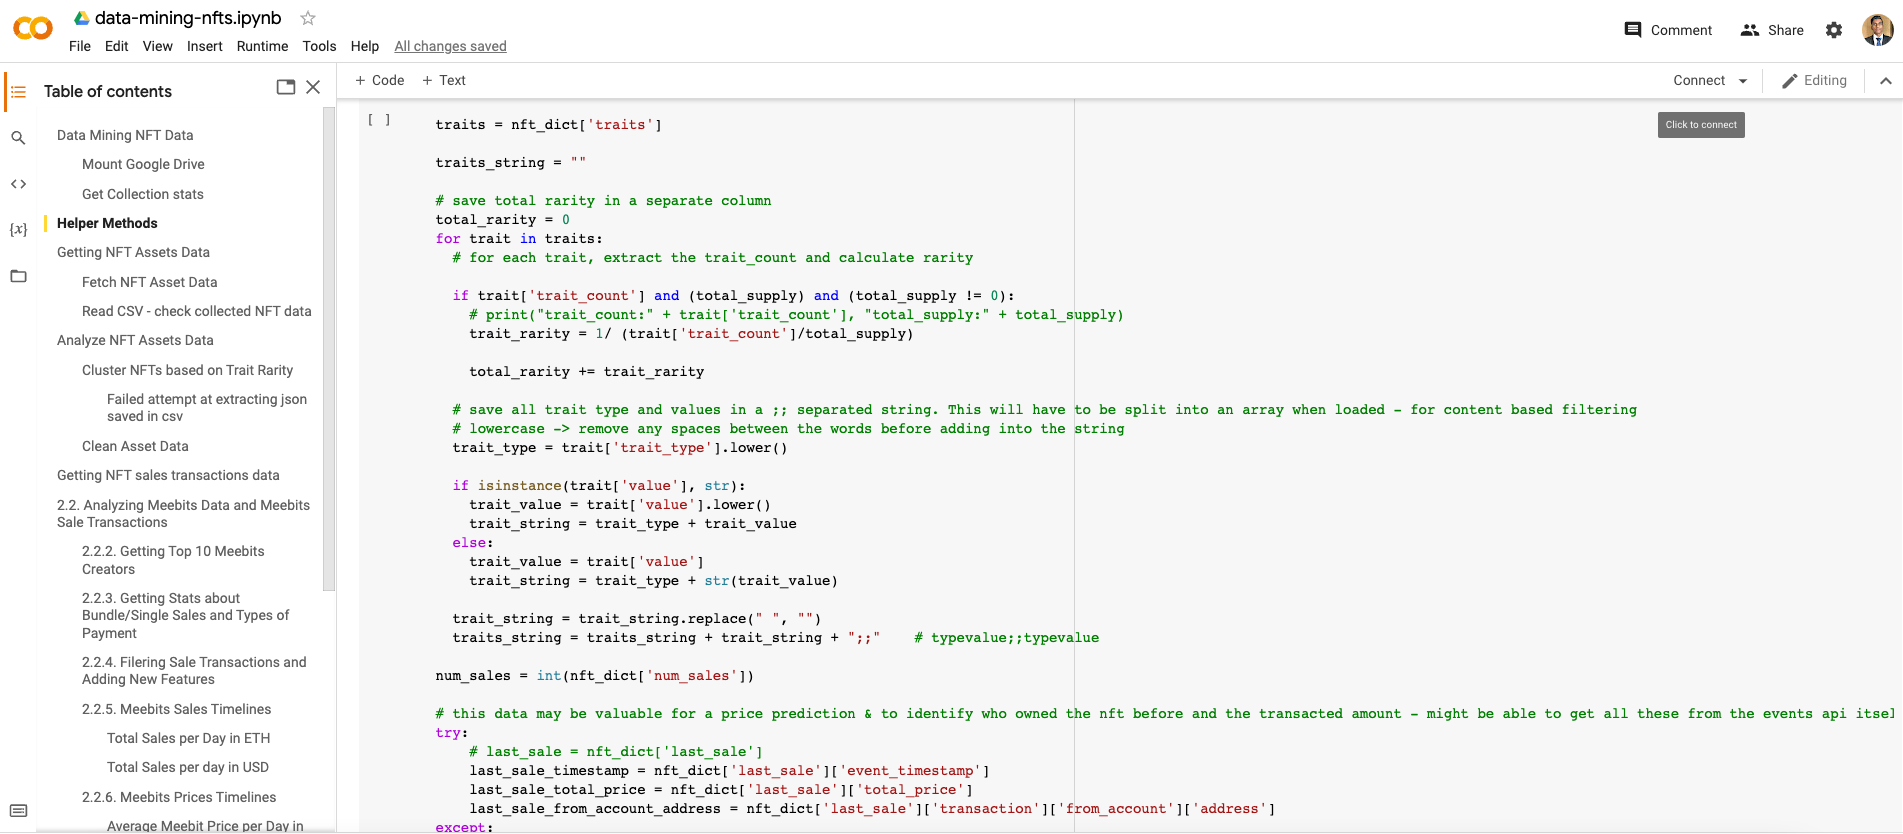
\includegraphics[width=0.95\textwidth]{images/Implementation/code/nft-data-extraction.png}
\caption{Implementation code segment: \gls{nft} data mining \& preprocessing \textit{(self-composed)}}
\label{fig:code-nft-data-mining}
\end{figure}

\vspace{-6mm}
The data extraction is done to extract information required for recommendations, to view details of items \& to save information for recommendation algorithms/ predictions that are potentially possible in the future.

\subsubsection{\gls{nlp} Preprocessing, Vectorizing \& Recommendations}

%  -- using a countvectorizer with reasoning
\begin{figure}[h!]
\centering
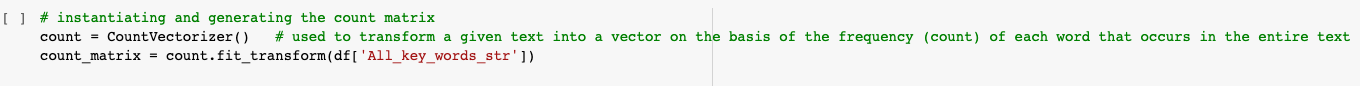
\includegraphics[width=0.95\textwidth]{images/Implementation/code/content vectorizer.png}
\caption{Implementation code segment: Content Vectorizer \textit{(self-composed)}}
\label{fig:code-content-vectorizer}
\end{figure}

A Count Vectorizer was used from the \textit{scikit learn} library to vectorize all words, to be used for similarity matching. The reason for choosing the Count Vectorizer over a Tf-Idf Vectorizer was because Tf-Idf will give lower scores to more common words found in the dataset. Since our intent is to identify all the possible matches and primarily rank the content based results using global trends, it made more sense to go with a Count Vectorizer.

% generating a cosine similarity matrix
\begin{figure}[h!]
\centering
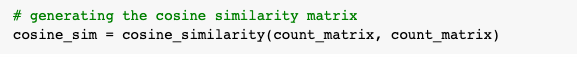
\includegraphics[width=0.95\textwidth]{images/Implementation/code/cosine-matrix.png}
\caption{Implementation code segment: Generating the Cosine Similarity Matrix \textit{(self-composed)}}
\label{fig:code-cosine-matrix}
\end{figure}
A Cosine Similarity Matrix is then generated from the \textit{scikit learn} library to identify all the matching words contained across all \gls{nft}s content. This generates the recommendation ahead of time.

% -- matching using trends
% -- matching using trait-rarity - trait-rarity recommendations
\begin{figure}[h!]
\centering
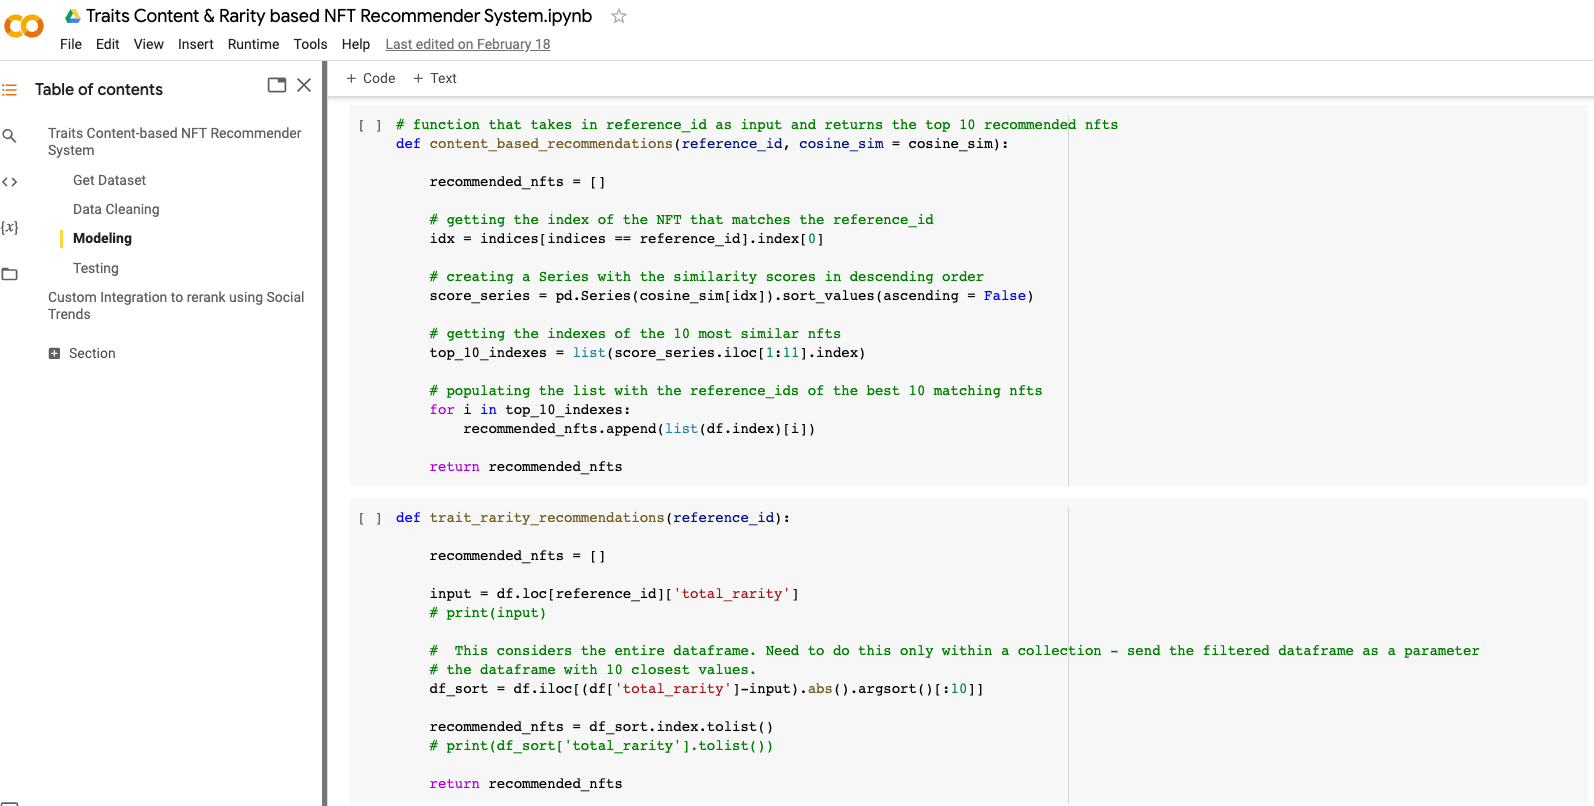
\includegraphics[width=0.95\textwidth]{images/Implementation/code/trait-rarity recommendations.png}
\caption{Implementation code segment: Produce Trait Rarity Based Recommendations \textit{(self-composed)}}
\label{fig:code-trait-rarity-rec}
\end{figure}

The above recommendation generation algorithms were created to cater towards matching \gls{nft}s within a collection, since most of the major \gls{nft}-collections have comparatively more unique data in traits compared to descriptions. Trait rarity similarity was identified to be the best way to identify total uniqueness which represents the value of each \gls{nft}. Although the calculation of total rarity was explored by \textit{rarity tools} during the course of the research, recommending similar total rarities is a novel implementation in the application domain.

\subsubsection{Trends Extraction, Preprocessing \& Recommendations}
% trends data preprocessing
% preprocessing trends
\begin{figure}[h!]
\centering
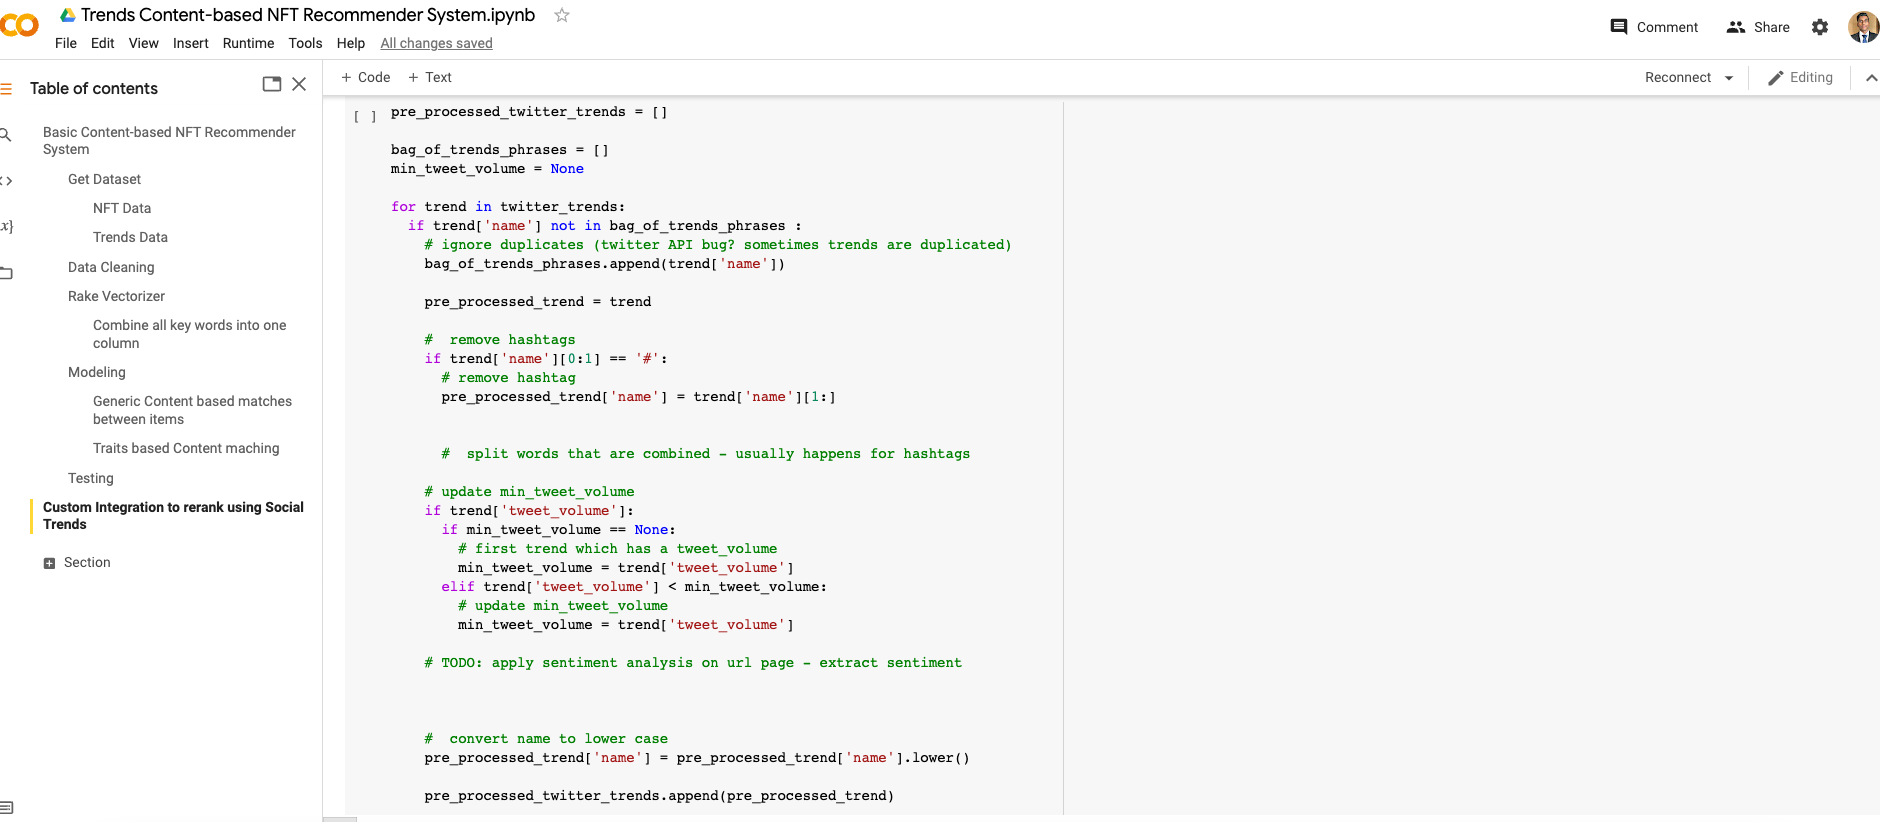
\includegraphics[width=0.95\textwidth]{images/Implementation/code/preprocessing trends.png}
\caption{Implementation code segment: Preprocess Trends Data \textit{(self-composed)}}
\label{fig:code-preprocess-trends}
\end{figure}

The above code segment preprcoesses trends that are fetched from the live Twitter \gls{api}.

% tweet volume extraction
\begin{figure}[h!]
\centering
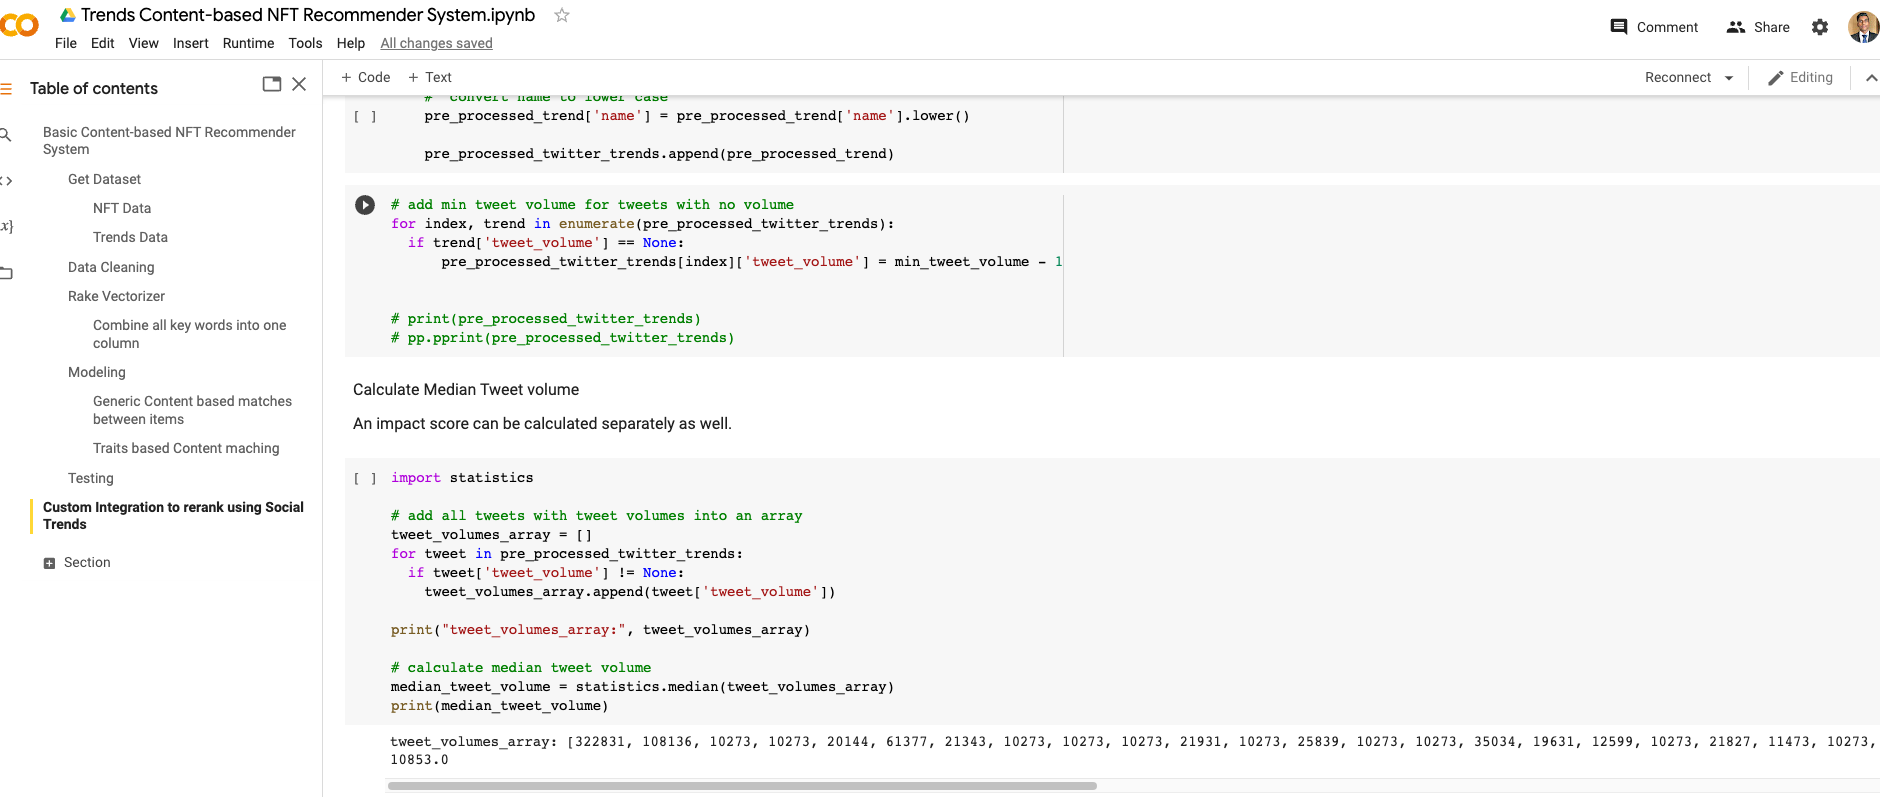
\includegraphics[width=0.95\textwidth]{images/Implementation/code/tweet-volume calculation.png}
\caption{Implementation code segment: Calculating Trends Score \textit{(self-composed)}}
\label{fig:code-tweet-volume-extraction}
\end{figure}

The above code segment assigns a tweet volume for trends with no volume \& calculates the median Tweet volume which used to calculate the impact score of each trend.

% calculating trends score for trends based recommendations
The below code segment is used to calculate the trends score for each \gls{nft} and finally make trends-based recommendations.
\begin{figure}[h!]
\centering
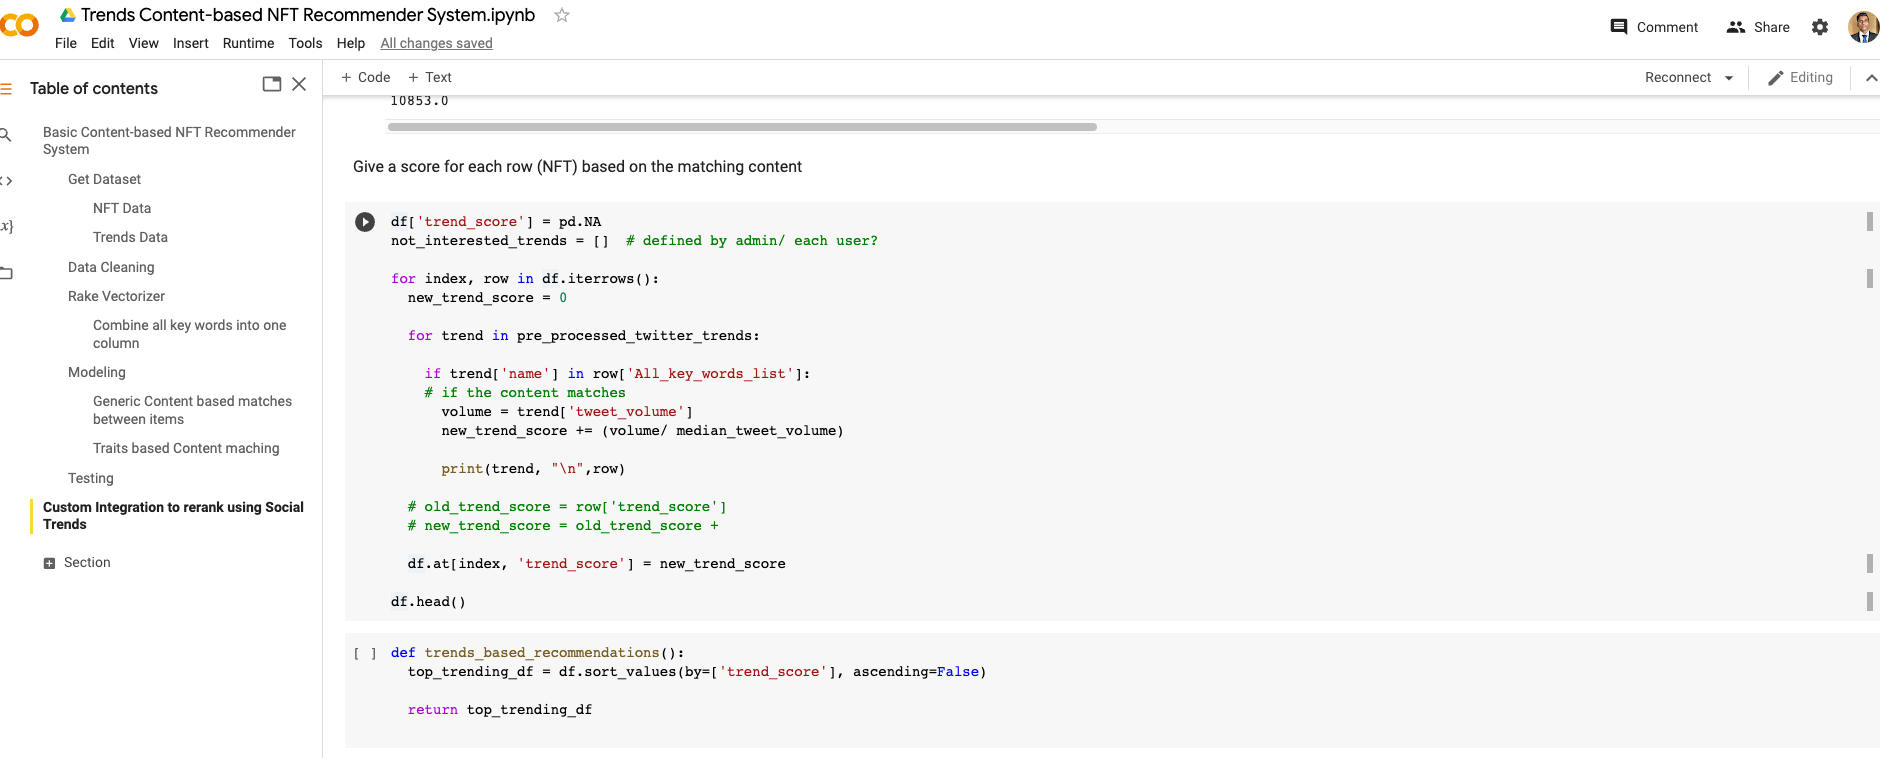
\includegraphics[width=0.95\textwidth]{images/Implementation/code/calculating trends score.png}
\caption{Implementation code segment: Calculating Trends Score \textit{(self-composed)}}
\label{fig:code-trends-score}
\end{figure}

% ensembling

\section{User Interface}

The UI wireframes depicting the planned UI for the MVP (Minimum Viable Product) have been place in \textbf{\nameref{appendix:UI-Wireframes}}.

\section{Self-Reflection}
% reflection on your current prototype.
The current prototype implementation covers the core research component focused in the research, but there are points of improvements that the author would like to achieve before the end of the final prototype. The use of multiple data sources for trends is something that can be added as a plugin, to increase the trends-score and find more matches for trends based recommendations. Showing how the results vary across time would also be better to be shown when evaluating the novel architecture. Furthermore, the utilization of item-to-item collaborative filtering and price prediction would be interesting to be explored, to complete \& present the recommendations ecosystem that is possible to be created with the suggested design architecture.

Prior to adding more models to the system, the author's primary goal in implementation over the next few weeks would be to implement the front-end, \gls{api} proxy and database connection to present a completed, user-friendly minimum viable product.

Considering the tight deadline and time-constraint to achieve a completed core research component, the level of completion of the prototype together with the research documentation is extremely satisfactory.
% Results of evaluation metrics and if possible also have the qualitative evaluation - check across a time period, how the recommendations vary and appear to be timely compared to recommendations produced without integrating social trends.

Embarrassing concepts of Decentralized Systems \& paving the path to Web 3.0, the research contribution brought forward in this project is expected to open up even more possibilities with time.

\section{Video Demo}
% Upload video to Youtube as unlisted video and provide Link to video demo
The link to the demo video presenting the current implementation progress can be found here: \url{https://youtu.be/drfU3h3LndQ}

\section{Chapter Summary}
The chapter comprised of the technologies, languages \& supporting tools utilized to implement the prototype developed as part of the research. Discussions accompany the code snippets and algorithms produced as part of core functionality. Finally, the author's self-reflection of the developed prototype was presented.
